\documentclass{article}
    \author{杨铭\\5130379022}
    \title{魁地奇桌球 - 第二次迭代}
\usepackage{ctex}
\usepackage{graphicx}
\usepackage{color}
\usepackage{listings}
\usepackage{xcolor}
    \definecolor{gray}{rgb}{0.9,0.9,0.9}
\begin{document}
\lstset{numbers=left,
numberstyle=\tiny,
keywordstyle=\color{blue!70}, commentstyle=\color{red!50!green!50!blue!50},
frame=shadowbox,
rulesepcolor=\color{red!30!green!30!blue!30}
}
    \maketitle
    \section{开发环境}
        \begin{description}
          \item[操作系统] windows7旗舰版
          \item[开发软件] Visual Studio 2015 community
          \item[图形库] OpenGL:gl、glut、glaux
        \end{description}
    \section{简述}
        \paragraph{}
        在第一次迭代的基础上,进行了旗帜的建模,使用opengl完成了下列功能:
        \begin{itemize}
          \item 加入了光照效果
          \item 用各种曲线函数设计并构建旗帜模型
          \item 在旗帜模型上加入自己独特的贴图
          \item 在旗帜模型中加入旗帜飘扬的相关动画
        \end{itemize}
    \section{实现过程}
        \subsection{概括}
        \paragraph{}
        在工程中新建了\textbf{flag.h,flag.cpp,glhf.h,glhf.cpp}四个文件,在\textbf{flag.h} 和\textbf{flag.cpp}中定义并实现了旗帜类,在\textbf{glhf.h}中包含了opengl的一些核心库和辅助库并且为读取纹理包装了一个函数
        \subsection{读取纹理}
            \paragraph{}
            使用glaux库的AUX\_RGBImageRec类读取文件并且使用glTexImage2D函数将纹理映射到内存中
        \subsection{旗帜绘制}
            \begin{lstlisting}[language={[ANSI]C}]
class Flag
{
public:
  Flag();

  void init();
  void render();
  void update();
	
  void setWind(int level);
  void windUp();
  void windDown();

private:
  GLfloat ctrlPoints[X_CTR_NUM][Y_CTR_NUM][3];
  GLfloat texpts[2][2][2];
  GLuint tex_ID;
  GLfloat dt;
  int w_level;
  GLfloat post_length, post_radius;
  GLfloat y_d, y_offset;
};
            \end{lstlisting}
            \paragraph{说明}
            类似其他的实体类,主要方法为init、render、update分别实现初始化、绘制和更新数据。
            成员变量中包含两个3维数组\textbf{ctrlPoints}、\textbf{texpts},分别为旗帜的曲面控制点和纹理的映射点。
            \textbf{tex\_ID}保存着之前为旗帜读取的纹理的编号\textbf{dt}是旗帜更新的时间间隔。\textbf{w\_level}记录模拟风力的大小,
            它影响着\textbf{y\_d}、\textbf{y\_offset},从而影响旗帜飘动的频率、幅度和y轴偏移量,
            可以通过调用\textbf{setWind}、或者\textbf{windUp}、\textbf{windDown}来调节风力大小
            \paragraph{绘制}
            在render函数中,使用opengl的二维差值器,实现了贝塞尔曲线的旗帜绘制和纹理贴制。
            \begin{lstlisting}[language={[ANSI]C}]
void Flag::render()
{
  glMatrixMode(GL_MODELVIEW);

  // draw flagpole
  glPushMatrix();
  glTranslatef(0.0f, 24.0f, 0.0f);
  glColor3f(0.5f, 0.25f, 0.0f);
  GLUquadric *pObj;
  pObj = gluNewQuadric();
  gluCylinder(pObj, post_radius,
              post_radius, post_length, 12, 1);
  glPopMatrix();

  // draw flag
  glPushMatrix();

  glTranslatef(3.8f, 24.0f, 8.5f);
  // bind texture id
  glBindTexture(GL_TEXTURE_2D, tex_ID);
  // enable 2D texture and 2D calculator to draw surface
  glEnable(GL_TEXTURE_2D);
  glEnable(GL_MAP2_VERTEX_3);
  glEnable(GL_MAP2_TEXTURE_COORD_2);
  
  glMap2f(GL_MAP2_VERTEX_3,0.0f,10.0f,3,5,
          0.0f,10.0f,15,2,&ctrlPoints[0][0][0]);
  glMap2f(GL_MAP2_TEXTURE_COORD_2,0.0f,10.0f,2,2,
          0.0f,10.0f,4,2,&texpts[0][0][0]);
  glMapGrid2f(10, 0.0f, 10.0f, 10, 0.0f, 10.0f);

  glTexEnvf(GL_TEXTURE_ENV, GL_TEXTURE_ENV_MODE,
            GL_DECAL);
  glEvalMesh2(GL_FILL, 0, 10, 0, 10);
  glPopMatrix();

  glutSwapBuffers();
  glDisable(GL_TEXTURE_2D);
}
            \end{lstlisting}
            \paragraph{更新}
            在update里更新控制点的坐标,用三角函数模拟旗帜迎风飘动的效果\\
            本来想使用质点-弹簧模型的布料模拟,但是时间所限导致实现效果不理想,暂时使用这种方式模拟旗帜的物理模型
        \subsection{光照}
            \paragraph{}
            在\textbf{main.cpp}中的\textbf{initlights}中开启光照效果\\
            首先开启光照效果和材质反光和颜色反光,设置环境光和光源位置、漫反射光和镜面发射等属性
            \begin{lstlisting}[language={[ANSI]C}]
void initlights(void)
{
  GLfloat ambient[] = { 0.2, 0.2, 0.2, 1.0 };
  GLfloat position[] = { 0.0, 0.0, 2.0, 1.0 };
  GLfloat mat_diffuse[] = { 0.6, 0.6, 0.6, 1.0 };
  GLfloat mat_specular[] = { 1.0, 1.0, 1.0, 1.0 };
  GLfloat mat_shininess[] = { 50.0 };
  glEnable(GL_LIGHTING);
  glEnable(GL_LIGHT0);
  glEnable(GL_COLOR_MATERIAL);
  glEnable(GL_AUTO_NORMAL);
  glLightfv(GL_LIGHT0, GL_AMBIENT, ambient);
  glLightfv(GL_LIGHT0, GL_POSITION, position);
  glMaterialfv(GL_FRONT, GL_DIFFUSE, mat_diffuse);
  glMaterialfv(GL_FRONT, GL_SPECULAR, mat_specular);
  glMaterialfv(GL_FRONT, GL_SHININESS, mat_shininess);
}
            \end{lstlisting}
    \section{结果展示}
        \begin{figure}[bhtp]
                \begin{minipage}[bhtp!]{1\linewidth}\centering
                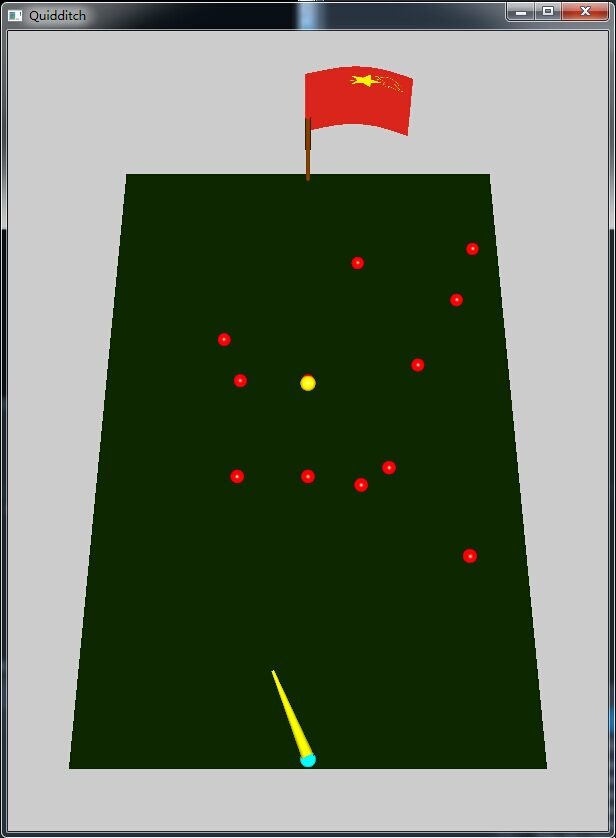
\includegraphics[width=9cm]{result.jpg}
                \caption{效果图}\label{1-a}
                \end{minipage}
        \end{figure}

\end{document}
